\documentclass{sigchi}

% Use this command to override the default ACM copyright statement (e.g. for preprints). 
% Consult the conference website for the camera-ready copyright statement.


%% EXAMPLE BEGIN -- HOW TO OVERRIDE THE DEFAULT COPYRIGHT STRIP -- (July 22, 2013 - Paul Baumann)
% \toappear{Permission to make digital or hard copies of all or part of this work for personal or classroom use is 	granted without fee provided that copies are not made or distributed for profit or commercial advantage and that copies bear this notice and the full citation on the first page. Copyrights for components of this work owned by others than ACM must be honored. Abstracting with credit is permitted. To copy otherwise, or republish, to post on servers or to redistribute to lists, requires prior specific permission and/or a fee. Request permissions from permissions@acm.org. \\
% {\emph{CHI'14}}, April 26--May 1, 2014, Toronto, Canada. \\
% Copyright \copyright~2014 ACM ISBN/14/04...\$15.00. \\
% DOI string from ACM form confirmation}
%% EXAMPLE END -- HOW TO OVERRIDE THE DEFAULT COPYRIGHT STRIP -- (July 22, 2013 - Paul Baumann)


% Arabic page numbers for submission. 
% Remove this line to eliminate page numbers for the camera ready copy
% \pagenumbering{arabic}


% Load basic packages
\usepackage{balance}  % to better equalize the last page
\usepackage{graphics} % for EPS, load graphicx instead
\usepackage{times}    % comment if you want LaTeX's default font
\usepackage{url}      % llt: nicely formatted URLs

% llt: Define a global style for URLs, rather that the default one
\makeatletter
\def\url@leostyle{%
  \@ifundefined{selectfont}{\def\UrlFont{\sf}}{\def\UrlFont{\small\bf\ttfamily}}}
\makeatother
\urlstyle{leo}


% To make various LaTeX processors do the right thing with page size.
\def\pprw{8.5in}
\def\pprh{11in}
\special{papersize=\pprw,\pprh}
\setlength{\paperwidth}{\pprw}
\setlength{\paperheight}{\pprh}
\setlength{\pdfpagewidth}{\pprw}
\setlength{\pdfpageheight}{\pprh}

% Make sure hyperref comes last of your loaded packages, 
% to give it a fighting chance of not being over-written, 
% since its job is to redefine many LaTeX commands.
\usepackage[pdftex]{hyperref}
\hypersetup{
pdftitle={SIGCHI Conference Proceedings Format},
pdfauthor={LaTeX},
pdfkeywords={SIGCHI, proceedings, archival format},
bookmarksnumbered,
pdfstartview={FitH},
colorlinks,
citecolor=black,
filecolor=black,
linkcolor=black,
urlcolor=black,
breaklinks=true,
}

% create a shortcut to typeset table headings
\newcommand\tabhead[1]{\small\textbf{#1}}


% End of preamble. Here it comes the document.
\begin{document}

\title{Crowdsourcing on In-building Routing System with Personal Preferences across Building Groups}

\numberofauthors{3}
\author{
  \alignauthor Junnan CHEN\\
    \affaddr{Waterloo, Canada}\\
    \email{j486chen@uwaterloo.ca}\\
  \alignauthor Henagzhi ZHANG\\
    \affaddr{Waterloo, Canada}\\
    \email{h246zhang@uwaterloo.ca}\\
}

\maketitle

\begin{abstract}
People travel inside building groups from a room in building A to another in building B frequently. Traditional routing system usually provides shortest routes between two coordinates consist of longitudes and latitudes, but does not have knowledge about building structures and detailed floor maps. It does not take users' personal preferences into account when suggesting the routes as well. Such routes generated cannot meet people’s demand. In this paper, we introduce a new system, which provides in-building routes with personal preferences across building groups.
\end{abstract}

\keywords{
	Crowdsourcing; In-building Routing; Personal Preferences; Mobile Interfaces; Concept of Association; Decision Tree.
}

\section{Introduction}

introduction
In our world, most people are living, working or studying in a group of buildings which could be company buildings, neighbourhoods or campus buildings. People go from one location inside the building-group to another every hour every day. Traditional route planning system provides routes between two coordinates consist of longitudes and latitudes, focusing on finding the shortest route, but does not have knowledge about the inside structures of buildings and floor-detailed environments, and does not take users' personal perferences into account when suggesting the routes. Those routes cannot provide enough details and personal options demanded by people.
For example, an employee may need to go to the coffee shop on the first floor of building B from his office on the third floor of building A several times a day. His route choices would be based on the weather condition and his physical condition. He would choose to go through the hallway between the two buildings if it rained or take the elevator if he feels tired. Traditional route planning system would only provide the shortest route from the exit of building B to the entrance of building A regardless of the building structures or floor environments, which cannot meet this employee's actual needs.


Here we want to introduce a new in-building routing system with persoanl preferences, a system with comprehensive knowledge of building structures, floor-level detailed maps, and relevant environments, which provides room-level detailed routes with personal preferences specified by the user. The focus of this system would be mapping the physical features of routes to human preferences which consist of physical requirement, personal feelings, emotional options and etc. The system shall collect route and preference data from people, and then analyze the relationships between human preferences and physical features.


Our system collect the trainning data, which are actual routes each has its personal preferences labeled, by crowdsourcing methods. Crowdsourcing has been successfully used in many fields. We provide an application on mobile devices, which encourages people to record their daily routes from one room location to another across building groups. Before they start to record routes, the application will ask the user about their personal feelings today (e.g. Are you hurry now? or Are you feeling tired now?), their special demands for the following route (e.g. Will you pass Tim Hortons on your way? or Do you need to use the bathroom on your way?) as well as some weather conditions (e.g. Is it sunny out side? or Is it snowing now?). Once the users finish the questionares, they will be presented an interface for them to record their routes. During the recording process, the application collects physical data of the route in the form of points on the floor map inputted by the user. 


Our system will analyse the routes collected and the corresponding physical features of a particular route (e.g. the number of stairs, number of turns) with personal preferences such as physical requirement, personal feelings, and emotional options provided by the user. We will construct our model using the concept of decision tree. The model is trained by the collected data and will be able to predict the best route given a set of personal preferences.


Our final product aims to generate the proper routes upon request. Using this product, the user could specify two room locations, together with one or more personal preferences. Then, the system will run the model and return the most satisfying route. The system will display the route on the screen for the user. 


In this paper, we describe the design of the courdsourcing routes collecting method, the feature analysing method and route generating system. We test the system with University of Waterloo campus building groups. We provide the test results, the detailed evaluation of our system and the future work.


\section{RELATED WORK}

During the system design process, we reviewed literature related to our ideas. The Kimono ~\cite{huang2005kimono} is a knowledge sharing system, which presents the concept of association. Our in-building routing system uses this idea as well; for example, each route collected in the crowdsourcing stage is associated with a set of personal preferences specified by the user. One of the prior works we reviewed has the similar idea since it [4] includes a physical kiosk as well. In addition, the physical kiosks [4] are used for crowdsourcing. Since our system collects in-building routes with personal preferences from our users, crowdsourcing plays a significant role here, and crowdsourcing needs to be studied from the prior work [1, 2, 6]. Since our system requires users to record routes on the map displayed on the screen and provide inputs through the questionnaire, user interface designs need to be taken into our consideration. Some prior works [5, 7] provide us with very helpful results for our system design. Our results are based on decision trees. In order to have some insights about decision trees, we reviewed and studied related work [8, 9]. In this section, we discuss how prior work helps us develop our in-building routing system with personal preferences across building groups. 


\subsection{Concept of Association}

The Kimono paper ~\cite{huang2005kimono} presents a system, which extends the function of an information kiosk. The method they used in order to achieve the extension is to allow interactions between a kiosk and a mobile device, such as a smartphone. We know that a kiosk is usually a physically located machine displaying information. A user could stand in front of a kiosk, and touch the screen to select information of his or her interest. The information from the kiosk is relevant to the particular event at its location. Some disadvantages of a kiosk can be seen. For example, the kiosk lacks mobility, and it’s difficult to add more information to it.


To conquer these inflexibilities, the main idea introduced in the paper ~\cite{huang2005kimono} is to allow interactions between a mobile device (such as a smartphone) and a kiosk. People are familiar with smartphones as they use phones every day. Functionalities of a smartphone include taking pictures, taking notes, recording voices, and so on. Through these various ways, a person can easily create new contents at any time at his or her current location. Then he or she can associate the newly created contents with other selected contents or events presented on the kiosk. By uploading the new contents and its associations, other people can therefore have access to them.


The Kimono system ~\cite{huang2005kimono} described in the paper is designed specifically for researchers attending a conference. A number of kiosks are placed in the lobby of the conference. They all display the same information relevant to the event, such as conference locations, routes to the airport, hotels, etc. Changes of talk schedules and meal plans are posted on the kiosks as well. Participants of the conference use the touch panel display of a kiosk to select information interested in. Then the information selected is transferred to his or her smartphone. On the smartphone, the program will alert the user about the next event and other relevant details such as starting/ending time, room location, routes to the destination, etc.


While attending a lecture at the conference, one can use their smartphones to record notes in the form of text, image, video, or audio. Then they associate newly created notes with selected event or items such as papers or posters presented at the conference. People can also exchange notes with each other directly between two mobile devices, or post the notes they took on the kiosk. For those users who previously downloaded information from the kiosk to their smartphones, if the information downloaded has changed, the updates will be copied to the mobile devices through the system when the next synchronization occurs. 


The main insight we learned from the Kimono ~\cite{huang2005kimono} is the concept of associations, which makes the organization of data and synchronization much more simple. Users can get information of his or her interest displayed on the screen and associated information on the smartphone. New information can be created by the user, associated with other relevant information, and made available to others.


For our in-building routing system with personal preferences across building groups, the concept of association is utilized. During the crowdsourcing stage, users record their routes while walking to the destination, and later associate personal preferences or features with the route they just recorded. Personal preferences in our system include physical requirements, personal feelings, emotional options, etc. By associating personal preferences with the routes, the system could provide in-building routes with particular personal preferences specified by a user, and later collect ratings from the user about the routes suggested. 

\subsecton{Crowdsourcing}

We can see that a lot of researches and experiments are conducted in prior works [4, 6] in the area of crowdsourcing. Here we discuss the paper [4], in which crowdsourcing concepts are presented and extended as communitysourcing. What we know is that crowdsourcing involves division and assignment of tasks to a number of online users. In order to have better quality work, the kiosk is used to attract the right crowds to perform tasks. In this case, the right crowds are required to be knowledgeable enough in the corresponding task domain assigned to them. The result the paper showed is that the crowdsourcing system was able to perform the grading task more accurately than traditional grading.


What we did is to incorporate the idea of crowdsourcing into our system. That is, we let crowds generate routes with personal preferences through our system. As the system provides in-building routes across building groups on campus, the potential crowds we are interested in are students, teachers, and staffs. One reason is that they are familiar with the building structures and floor-detailed environments, and therefore the quality of crowdsourced routes is greatly improved. Another reason is that we could obtain enough route data in a relatively short period of time through the crowdsourcing stage. Furthermore, during the crowdsourcing stage, the system could capture a particular set of preferences associated with a route, and later suggest this route upon requests of same or similar preferences in the set.


\subsection{User Interface}

Since we require the routes to be recorded when users walk to their destinations, our system provides an interface on both computers and mobile devices. The user gets access to our system on the screen in the beginning of his or her journey. Partial map centered at his or her current position is displayed. The user periodically marks his or her next new position along the way to the destination, and the map accordingly centers at the newly marked position. A questionnaire is displayed to request his or her personal preferences associated with the recorded route before the user starts recording.


The questions on the questionnaire are asked before the recording process. The questionnaire of our system helps to collect the personal preference data with the crowdsourced routes of our interest. After thinking of what kinds of questions should be asked, we have the questions such as the weather conditions, the fatigue level, pass coffee shop or not, hurry level, and etc.


When designing such a crowdsourcing interface, we need to think about whether our user interface or task design is effective on both computers and mobile devices. We reviewed the prior paper [5] to gain better understandings and insights about crowdsourcing user interfaces and task designs for mobile users.


The main question in the paper [5] the author trying to answer is “Which crowdsourcing platforms and which kinds of tasks are more adequate to mobile devices”. It turns out that some of those inadequacy issues are superficial, and they can be resolved by providing better user interfaces and/or better crowdsourcing task designs. Several typical reasons for such inadequacy issues on mobile phones are found as well, such as redundant task description, unsupported formats of audio, scrolling problem, layout problem in a small display, and so on.  


For our system, we also try to conquer these problems by designing simple tasks, requesting simplified inputs, providing concise interfaces, etc. Our system knows the building structures and all of the floor maps. Users records routes through their mobile devices while walking. Partial map centered at the current position is showed, and the user marks the next point along the journey. Upon request of a route with personal preferences specified by a user, the system provides in-building routes and collects ratings for the suggested route afterwards. Several benefits can be seen in our system. For example, instead of keeping track of the entire route walked, the user only needs to mark the next new point by touching the screen every time they move as the partial map will always centered at his or her current point. After gathering point information inputted by the user, the system itself can generate the corresponding route. By displaying only the partial map instead of the entire floor map, we successfully resolve the bad layout problem on small portable screens.


\subsection{Decision Tree}

Our results are based on decision trees. As described in the previous section, our system provides users with an interface through which users perform question answering and route recording tasks. The system requires users to answer a questionnaire before they start to record their in-building routes during the crowdsourcing stage. The questionnaire here in the system is used to collect personal preference data associated with the routes recorded. And decision trees are then built accordingly. 


We built several graphs of decision trees. What we did was the review of several prior works [8, 9] involving the decision trees. A decision tree provides us with support in decision-making. It is known as a tool, which uses a tree like graph or model of decisions and their possible consequences. A decision tree is a useful technique, which learns a model from a provided data set inductively. In order to build a decision tree, we need to be clear about the structure of a decision tree. The tree structure consists of internal nodes, branches, and leaf nodes. We describe each of the above in turn. Each of the internal nodes is a test on an attribute from our crowdsourced data. Each of the branches represents the result from an internal node. Lastly, a leaf node can be seen as a class label. Three types of nodes are in a decision tree. They are decision nodes, chance nodes, and end nodes. The algorithm is shown to readers through a decision tree. 


Existing algorithms are introduced in early papers [10, 11] to help build decision trees. These algorithms [10, 11] build decision trees from the given set of training data. Top down structures are built, partitioning instances into different classes. The splits of instances are based on different attribute values. The algorithm from early work [10] uses Gini index to select the splitting attribute. The Gini impurity measures how often a random element from a data set is incorrectly labeled if it was randomly labeled according to the distribution of labels in the subset. Specifically, the Gini impurity is the summation of fi times (1-fi) where fi is the fraction of elements labeled with i.


Decision trees are traditionally drawn manually. However, they can grow to very large trees, which makes it difficult for a person to draw by hand. Here, we used a specialized package in Python to generate decision tree graphs for us. Our goal is to have a model that learns from the data gathered and later makes predictions on some variable of interest. In the graphs we created, colored nodes according to their classes together with explicit variable names are shown. 


Decision trees are commonly utilized in many analytical procedures. What we learned from prior work are a number of advantages of such a decision support technique as follows. For example, a decision tree is relatively easy to understand and interpret, and it requires little data preparation. Furthermore, it allows adding new cases, and can be combined with other decision support techniques. The cost of prediction on a targeted variable using the tree is logarithmic in the training data size.


\section{Typeset Text}

Prepare your submissions on a word processor or typesetter.  Please
note that page layout may change slightly depending upon the printer
you have specified.  \LaTeX\ sometimes will create overfull lines
that extend into columns.  To attempt to combat this, the .cls
file has a command, {\textbackslash}sloppy, that essentially asks
\LaTeX\ to prefer underfull lines with extra whitespace.  For more
details on this, and info on how to control it more finely, check out
{\url{http://www.economics.utoronto.ca/osborne/latex/PMAKEUP.HTM}}.

\subsection{Title and Authors}

Your paper's title, authors and affiliations should run across the
full width of the page in a single column 17.8 cm (7 in.) wide.  The
title should be in Helvetica 18-point bold; use Arial if Helvetica is
not available.  Authors' names should be in Times Roman 12-point bold,
and affiliations in Times Roman 12-point.  For more than three authors,
you may have to place some address information in a footnote, or in a named
section at the end of your paper. Please use full international addresses and
telephone dialing prefixes.  Leave one 10-pt line of white space below the last
line of affiliations.

\subsection{Abstract and Keywords}

Every submission should begin with an abstract of about 150 words,
followed by a set of keywords. The abstract and keywords should be
placed in the left column of the first page under the left half of the
title. The abstract should be a concise statement of the problem,
approach and conclusions of the work described.  It should clearly
state the paper's contribution to the field of HCI.

The first set of keywords will be used to index the paper in the
proceedings. The second set are used to catalogue the paper in the ACM
Digital Library. The latter are entries from the ACM Classification
System~\cite{acm_categories}.  In general, it should only be necessary
to pick one or more of the H5 subcategories, see
\url{http://www.acm.org/class/1998/ccs98.html}

\subsection{Normal or Body Text}

Please use a 10-point Times Roman font or, if this is unavailable,
another proportional font with serifs, as close as possible in
appearance to Times Roman 10-point. The Press 10-point font available
to users of Script is a good substitute for Times Roman. If Times
Roman is not available, try the font named Computer Modern Roman. On a
Macintosh, use the font named Times and not Times New Roman. Please
use sans-serif or non-proportional fonts only for special purposes,
such as headings or source code text.

\subsection{First Page Copyright Notice}

Leave 3 cm (1.25 in.) of blank space for the copyright notice at the
bottom of the left column of the first page. In this template a
floating text box will automatically generate the required space. Note
however that the text box is anchored to the \textbf{ABSTRACT}
heading, so if that heading is deleted the text box will disappear as
well.  You can replace the default copyright notice by uncommenting
the {\textbackslash}toappear block at the beginning of the document
and inserting your own text, for example, for versions under review.


\subsection{Subsequent Pages}

On pages beyond the first, start at the top of the page and continue
in double-column format.  The two columns on the last page should be
of equal length.

\begin{figure}[!h]
\centering
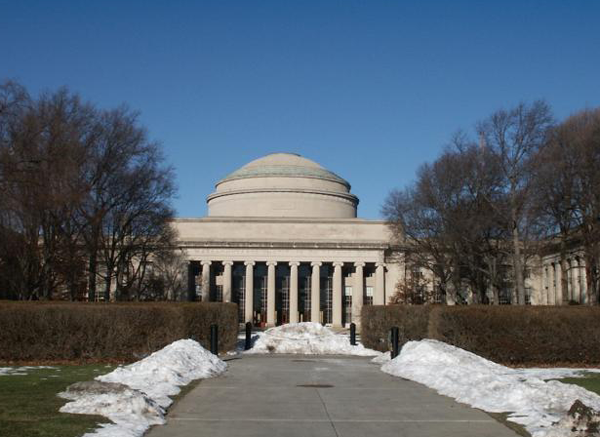
\includegraphics[width=0.9\columnwidth]{Figure1}
\caption{With Caption Below, be sure to have a good resolution image
  (see item D within the preparation instructions).}
\label{fig:figure1}
\end{figure}

\subsection{References and Citations}

Use a numbered list of references at the end of the article, ordered
alphabetically by first author, and referenced by numbers in brackets
\cite{ethics,
  Klemmer:2002:WSC:503376.503378,
  Mather:2000:MUT,
  Zellweger:2001:FAO:504216.504224}. For
papers from conference proceedings, include the title of the paper and
an abbreviated name of the conference (e.g., for Interact 2003
proceedings, use \textit{Proc. Interact 2003}). Do not include the
location of the conference or the exact date; do include the page
numbers if available. See the examples of citations at the end of this
document. Within this template file, use the \texttt{References} style
for the text of your citation.

Your references should be published materials accessible to the
public.  Internal technical reports may be cited only if they are
easily accessible (i.e., you provide the address for obtaining the
report within your citation) and may be obtained by any reader for a
nominal fee.  Proprietary information may not be cited. Private
communications should be acknowledged in the main text, not referenced
(e.g., ``[Robertson, personal communication]'').

\begin{table}
  \centering
  \begin{tabular}{|c|c|c|}
    \hline
    \tabhead{Objects} &
    \multicolumn{1}{|p{0.3\columnwidth}|}{\centering\tabhead{Caption --- pre-2002}} &
    \multicolumn{1}{|p{0.4\columnwidth}|}{\centering\tabhead{Caption --- 2003 and afterwards}} \\
    \hline
    Tables & Above & Below \\
    \hline
    Figures & Below & Below \\
    \hline
  \end{tabular}
  \caption{Table captions should be placed below the table.}
  \label{tab:table1}
\end{table}

\section{Sections}

The heading of a section should be in Helvetica 9-point bold, all in
capitals. Use Arial if Helvetica is not available. Sections should
not be numbered.

\subsection{Subsections}

Headings of subsections should be in Helvetica 9-point bold with
initial letters capitalized.  For
sub-sections and sub-subsections, a word like \emph{the} or \emph{of}
is not capitalized unless it is the first word of the heading.)

\subsubsection{Sub-subsections}

Headings for sub-subsections should be in Helvetica 9-point italic
with initial letters capitalized.  Standard {\textbackslash}section,
{\textbackslash}subsection, and {\textbackslash}subsubsection commands
will work fine.

\section{Figures/Captions}

Place figures and tables at the top or bottom of the appropriate
column or columns, on the same page as the relevant text
(see Figure~\ref{fig:figure1}). A figure or table may extend across both
columns to a maximum width of 17.78 cm (7 in.).

Captions should be Times New Roman 9-point bold.  They should be numbered (e.g.,
``Table~\ref{tab:table1}'' or ``Figure~\ref{fig:figure2}''), centered
and placed beneath the figure or table.  Please note that the words
``Figure'' and ``Table'' should be spelled out (e.g., ``Figure''
rather than ``Fig.'') wherever they occur.

Papers and notes may use color figures, which are included in the page
limit; the figures must be usable when printed in black and white in
the proceedings.  The paper may be accompanied by a short video figure
up to five minutes in length.  However, the paper should stand on its
own without the video figure, as the video may not be available to
everyone who reads the paper.

\section{Language, Style and Content}

The written and spoken language of SIGCHI is English. Spelling and
punctuation may use any dialect of English (e.g., British, Canadian,
US, etc.) provided this is done consistently. Hyphenation is
optional. To ensure suitability for an international audience, please
pay attention to the following:

\begin{itemize}
\item Write in a straightforward style.
\item Try to avoid long or complex sentence structures.
\item Briefly define or explain all technical terms that may be
  unfamiliar to readers.
\item Explain all acronyms the first time they are used in your text---e.g.,
``Digital Signal Processing (DSP)''.
\item Explain local references (e.g., not everyone knows all city
  names in a particular country).
\item Explain ``insider'' comments. Ensure that your whole audience
  understands any reference whose meaning you do not describe (e.g.,
  do not assume that everyone has used a Macintosh or a particular
  application).
\item Explain colloquial language and puns. Understanding phrases like
  ``red herring'' may require a local knowledge of English.  Humor and
  irony are difficult to translate.
\item Use unambiguous forms for culturally localized concepts, such as
  times, dates, currencies and numbers (e.g., ``1-5-97'' or ``5/1/97''
  may mean 5 January or 1 May, and ``seven o'clock'' may mean 7:00 am or
  19:00).  For currencies, indicate equivalences---e.g., ``Participants
  were paid 10,000 lire, or roughly \$5.''
\item Be careful with the use of gender-specific pronouns (he, she)
  and other gendered words (chairman, manpower, man-months). Use
  inclusive language that is gender-neutral (e.g., she or he, they,
  s/he, chair, staff, staff-hours,
  person-years). See~\cite{Schwartz:1995:GBF} for further advice and
  examples regarding gender and other personal attributes.
\item If possible, use the full (extended) alphabetic character set
  for names of persons, institutions, and places (e.g.,
  Gr{\o}nb{\ae}k, Lafreni\'ere, S\'anchez, Universit{\"a}t,
  Wei{\ss}enbach, Z{\"u}llighoven, \r{A}rhus, etc.).  These characters
  are already included in most versions of Times, Helvetica, and Arial
  fonts.
\end{itemize}

\section{Accessibility}
The Executive Council of SIGCHI has committed to making SIGCHI conferences more inclusive for researchers, practitioners, and educators with disabilities. As a part of this goal, the all authors are asked to work on improving the accessibility of their submissions. Specifically, we encourage authors to carry out the following five steps:
\begin{enumerate}
	\item Add alternative text to all figures
	\item Mark table headings
	\item Add tags to the PDF
	\item Verify the default language
	\item Set the tab order to ``Use Document Structure''
\end{enumerate}
Unfortunately good tools do not yet exist to create tagged PDF files from Latex. LaTeX users will need to carry out all of the above steps in the PDF directly using Adobe Acrobat, after the PDF has been generated.
 
For more information and links to instructions and resources, please see:
{\url{http://chi2014.acm.org/authors/guide-to-an-accessible-submission}}.

\section{Page Numbering, Headers and Footers}
Your final submission SHOULD NOT contain any footer or header string information 
at the top or bottom of each page. The submissions will be paginated in a determined 
order by the chairs and page numbers added to the pdf during the compiling, 
indexing, and pagination processes.

\section{Producing and Testing PDF Files}

We recommend that you produce a PDF version of your submission well
before the final deadline.  Your PDF file must be ACM DL
Compliant. The requirements for an ACM Compliant PDF are available at:
{\url{http://www.sheridanprinting.com/typedept/ACM-distilling-settings.htm}}.

Test your PDF file by viewing or printing it with the same software we
will use when we receive it, Adobe Acrobat Reader Version 7. This is
widely available at no cost from~\cite{acrobat}.  Note that most
reviewers will use a North American/European version of Acrobat
reader, which cannot handle documents containing non-North American or
non-European fonts (e.g. Asian fonts).  Please therefore do not use
Asian fonts, and verify this by testing with a North American/European
Acrobat reader (obtainable as above). Something as minor as including
a space or punctuation character in a two-byte font can render a file
unreadable.

\section{Blind Review}

For archival submissions, CHI requires a ``blind review.'' To prepare
your submission for blind review, remove author and institutional
identities in the title and header areas of the paper. You may also
need to remove part or all of the Acknowledgments text.  Further
suppression of identity in the body of the paper and references is
left to the authors' discretion. For more details, see the submission
guidelines and checklist for your submission category.

\section{Conclusion}

It is important that you write for the SIGCHI audience.  Please read
previous years' Proceedings to understand the writing style and
conventions that successful authors have used.  It is particularly
important that you state clearly what you have done, not merely what
you plan to do, and explain how your work is different from previously
published work, i.e., what is the unique contribution that your work
makes to the field?  Please consider what the reader will learn from
your submission, and how they will find your work useful.  If you
write with these questions in mind, your work is more likely to be
successful, both in being accepted into the Conference, and in
influencing the work of our field.

\section{Acknowledgments}

We thank CHI, PDC and CSCW volunteers, and all publications support
and staff, who wrote and provided helpful comments on previous
versions of this document.  Some of the references cited in this paper
are included for illustrative purposes only.  \textbf{Don't forget
to acknowledge funding sources as well}, so you don't wind up
having to correct it later.

% Balancing columns in a ref list is a bit of a pain because you
% either use a hack like flushend or balance, or manually insert
% a column break.  http://www.tex.ac.uk/cgi-bin/texfaq2html?label=balance
% multicols doesn't work because we're already in two-column mode,
% and flushend isn't awesome, so I choose balance.  See this
% for more info: http://cs.brown.edu/system/software/latex/doc/balance.pdf
%
% Note that in a perfect world balance wants to be in the first
% column of the last page.
%
% If balance doesn't work for you, you can remove that and
% hard-code a column break into the bbl file right before you
% submit:
%
% http://stackoverflow.com/questions/2149854/how-to-manually-equalize-columns-
% in-an-ieee-paper-if-using-bibtex
%
% Or, just remove \balance and give up on balancing the last page.
%
\balance

\section{References format}
References must be the same font size as other body text.
% REFERENCES FORMAT
% References must be the same font size as other body text.

\bibliographystyle{acm-sigchi}
\bibliography{sample}
\end{document}
